\chapter*{Introduction}
\label{cap:introduction}

\chapterquote{Los seres humanos no nacen para siempre el día en que sus madres los alumbran, sino que la vida los obliga a parirse a sí mismos una y otra vez}{Gabriel García Márquez}

\section{Motivation}
Over the years, video games have undergone a remarkable evolution, becoming increasingly complex. In parallel, enemies have evolved in the same way. In the specific context of two-dimensional platform games, enemies are more than mere opposition for the player—they are key to expressing the very essence of the game. Designing enemies, especially in this genre, is an ever more complex task. It is not limited to giving them a particular appearance; they must also exhibit unique behaviors and characteristics. As a result, the person entrusted with this task must possess multidisciplinary skills (art, design, programming, etc.).

In recent years, tools have emerged aimed at significantly streamlining the designers’ workflow. However, only a limited number of these focus specifically on this domain. The purpose of such tools is to ease the designer’s job, enabling them—even without programming expertise—to generate enemies with fully functional behaviors.

\section{Objectives}
The primary objective of this work is to design and develop a framework for the Unity game engine that simplifies and accelerates the creation of enemies in 2D platform games. This framework defines a modular structure of components and behaviors based on an analysis of common enemies in this genre, with the aim of completely separating the roles of programming and design. In doing so, it enables individuals without programming knowledge to take on the role of enemy designer.

As a practical demonstration of the framework, a functional Unity tool has been developed that allows users to implement and utilize these components in a visual and intuitive way. The tool includes an easy-to-use catalog of behaviors, as well as a user manual that clearly explains each component, its installation, and usage examples.

To carry out this development, a structured work plan was followed, covering everything from the environment study and review of existing enemies to the tool’s implementation, its validation with users, and the analysis of the obtained results.

\section{Work Plan}
This project follows the Scrum agile methodology, which creates a workflow focused on iteration and continuous improvement, ensuring efficient progress and the ability to adapt to issues as they arise. The work is divided into four main phases: research and planning, tool development, user testing, and thesis writing. Each phase is subdivided as follows:

\begin{itemize}
  \item \textbf{Research and Planning:}
    \begin{itemize}
      \item \emph{Problem Study:} In this initial phase, a state-of-the-art review will be conducted, focusing on the role of enemies in video games, their impact on gameplay, and the various techniques used in their design and behavior.
      \item \emph{Tool Selection and Analysis:} This phase involves a comparative analysis of different techniques and game engines, evaluating their advantages and disadvantages, as well as studying their architectures and workflows.
      \item \emph{Enemy Behavior Study:} This study will provide a solid foundation for the tool’s design by identifying common patterns in the behaviors of different enemies.
    \end{itemize}

  \item \textbf{Tool Development:}
    \begin{itemize}
      \item \emph{Design:} Define the proposed tool’s architecture, detailing the techniques employed, operation schemes, and organization of its main elements.
      \item \emph{Implementation of Core Features:} Develop the core functionalities for basic movements, including integration with sensors and actuators to enable interaction between them.
      \item \emph{Visual Aid Implementation:} Create visual aids intended to serve as references for designers, including graphical elements that facilitate understanding of behaviors.
      \item \emph{Testing and Debugging:} Carry out iterative tests to ensure the tool functions correctly, fixing any errors identified during implementation.
    \end{itemize}

  \item \textbf{User Testing:}
    \begin{itemize}
      \item Conduct tests with users who have not previously used the tool, following the plan detailed in Section~\ref{cap:evaluacionConUsuarios}. These tests will focus on uncovering potential issues with core features, validating functionality, and evaluating usability and clarity.
    \end{itemize}

  \item \textbf{Thesis Writing:}
    \begin{itemize}
      \item \emph{Initial Drafting:} Produce the initial draft covering all points specified in the thesis outline.
      \item \emph{Review and Revision:} Perform thorough reviews of the document and implement necessary corrections.
      \item \emph{Conclusions and Future Work:} After completing development and user testing, write the conclusions based on the results and outline possible future directions.
    \end{itemize}
\end{itemize}

\begin{figure}[h!]
  \centering
  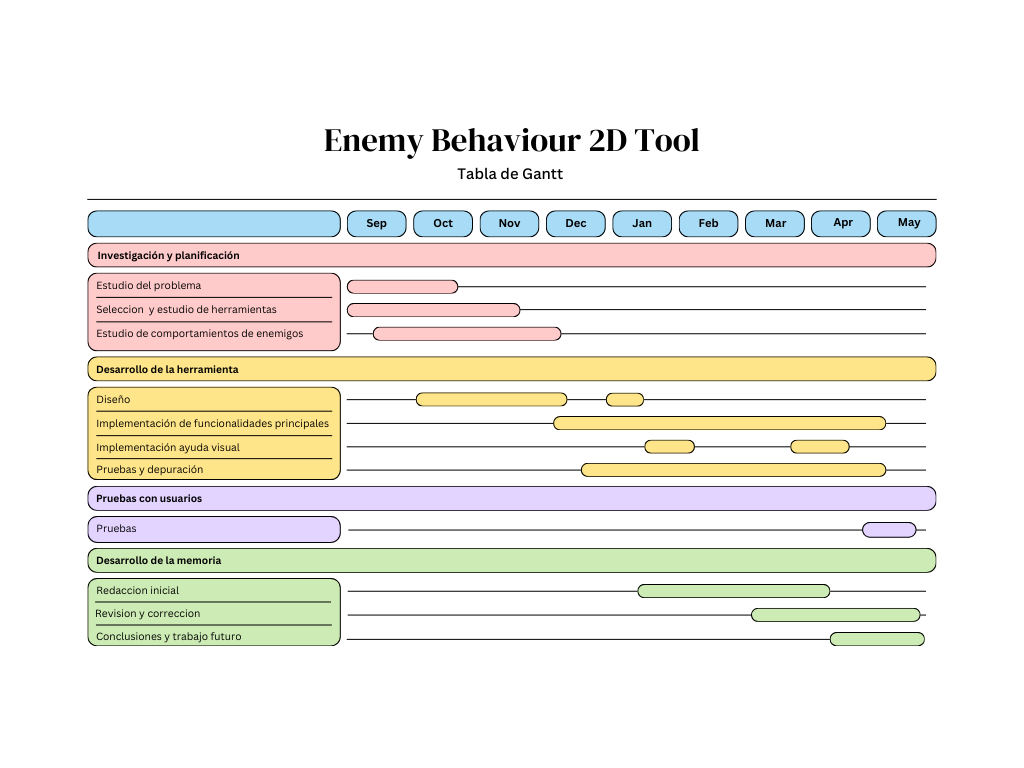
\includegraphics[height=12cm]{Imagenes/GanttChart}
  \caption{Gantt chart for the planning of the Enemy Behaviour 2D tool development}
  \label{fig:GanttEnemyBehaviour2D}
\end{figure}
